\documentclass[11pt,a4paper]{article}

% --- Minimal, VS Code friendly ---
\usepackage[utf8]{inputenc}
\usepackage[T1]{fontenc}
\usepackage[english]{babel}
\usepackage{geometry}
\geometry{margin=2.5cm}

\usepackage{lmodern}
\usepackage{microtype}
\usepackage[hidelinks]{hyperref}

% --- Math & units ---
\usepackage{amsmath,amssymb,mathtools}
\usepackage{siunitx}
\sisetup{detect-all, per-mode=symbol}

% --- Figures & tables ---
\usepackage{graphicx}
\usepackage{caption}
\usepackage{booktabs}

% --- Code listings ---
\usepackage{listings}
\lstset{
  basicstyle=\ttfamily\small,
  frame=single,
  breaklines=true,
  numbers=left,
  numberstyle=\tiny,
  tabsize=2,
  showstringspaces=false
}

% --- Metadata ---
\title{\textbf{MPM-Geomechanics Manual (v0.1)} \\
  \large MPM-Geomechanics: An open-source Material Point Method code for geomechanics.}
  \author{Dr. Fabricio Fernández}
\date{\today}

\begin{document}
\maketitle

\section{Introduction}
This is a minimal, VS Code--friendly LaTeX manual template.
Inline math like \( \sigma' = \sigma - u \) and display math:
$$
\frac{\partial \sigma_{ij}}{\partial x_j} + \rho\,b_i = \rho\,a_i.
$$

\section{ Introduction to the Material Point Method (MPM) }

The Material Point Method, or MPM, is a hybrid Lagrangian-Eulerian method that allows for simulating continuum mechanics processes involving large deformations and displacements without issues related to computational mesh distortion.
In MPM, the material domain to be simulated is discretized into a set of material points that can move freely within a computational mesh, where the equations of motion are solved.
The material points store all variables of interest during the simulation, such as stress, pore pressure, temperature, etc., giving the method its Lagrangian characteristic.

\begin{figure}[h]
  \centering
  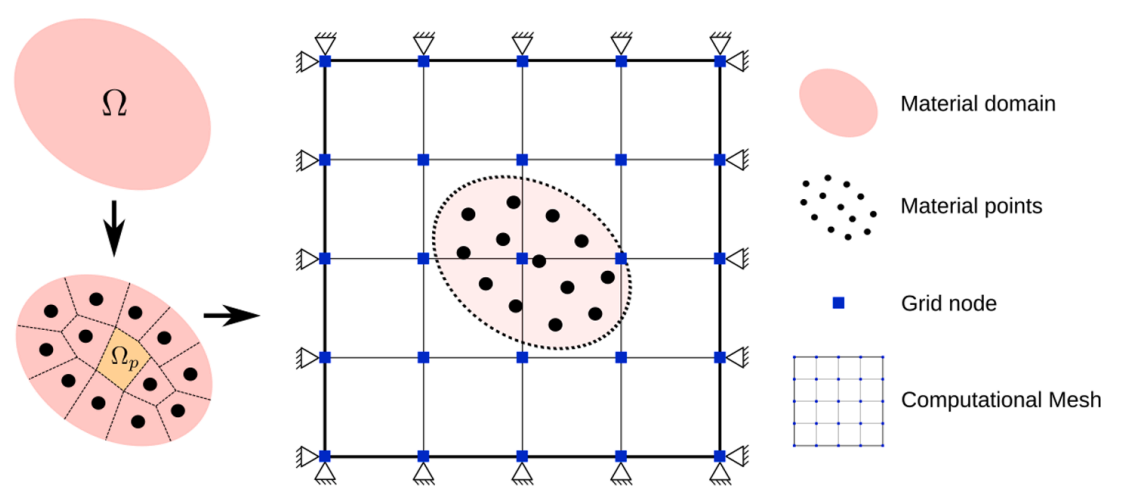
\includegraphics[width=\linewidth]{figures/mpm_discretization.png}
  \caption{MPM discretization: material points within a computational mesh.}
  \label{fig:mpm_discretization}
\end{figure}

In an MPM computational cycle, all variables stored in the material points are computed at the computational mesh nodes using interpolation functions, and then the equation of motion is solved at the nodes. The nodal solution obtained is interpolated back to the particles, whose positions are updated, and all nodal variables are discarded.

\begin{figure}[h]
  \centering
  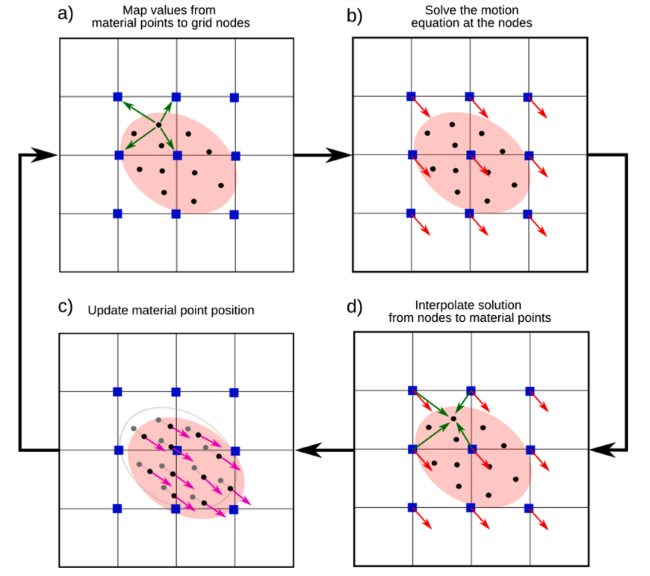
\includegraphics[width=.6\linewidth]{figures/mpm_cycle.png}
  \caption{MPM computational cycle.}
  \label{fig:mpm_cycle}

MPM Formulation

MPM enables the numerical solution of the equation of motion in continuum mechanics by using the nodes of an Eulerian mesh for integration and Lagrangian material points to transfer and store the properties of the medium.

The equation of motion in continuum mechanics

$$ \frac{\partial \sigma_{ij}}{\partial x_j} + \rho b_i = \rho a_i $$

where $\sigma_{ij} $ is the Cauchy stress tensor, $\rho$ is the density, $ b_i$ is the body force (regarding its mass), and $a_i$ is the acceleration of any point of the continuum.
Note that all equations are in tensor notation. So $a_i$ is the acceleration vector with tree dimensions in the space $x,y,z$.

The MPM formulation is obtained from the weak form of the motion equation and using a Petrov–Galerkin discretization scheme. The weak form of motion equation is obtained by multiplying the equation by arbitrary weighting functions, integrating this product over the domain, using integration by parts to reduce the order of the stress term and introducing the boundary conditions:

$$ -\int_{\Omega} \sigma_{i j} \delta u_{i, j} dV + \int_{\Gamma} t_i \delta u_i dA + \int_{\Omega} \rho b_i \delta u_i dV = \int_{\Omega} \rho a_i \delta u_i dV $$

here $\delta u_i$ are virtual displacements, whose value in the boundary are $\delta u_i |_{\Gamma} = 0$ and $t_i$ is an external traction acting on the boundary $\Gamma$.

In the MPM context any field or space property $f(x_i)$ can approximated using the value stored in the particle $f_p$:

$$ f(x_i) = \sum f_p \chi_p (x_i) $$

where $\chi_p$ is the particle characteristic function that defines the volume occupied by the material point:

$$ V_p = \int_{\Omega_p \cap \Omega} \chi_p(x_i) dV $$

consequently, in the MPM context, the density, the acceleration and the stress fields can be approximated by the values stored in particles:

$$ \rho(x_i) = \sum_p \frac{m_p}{V_{ip}} \chi_p(x_i) \rho(x_i) a_i(x_i) = \sum_p \frac{\dot{p_{ip}}}{V_p} \chi_p(x_i) \sigma_{i j}(x_i) = \sum_p \sigma_{i j p} \chi_p(x_i) $$

where $\dot{p_{ip}} = m_p \dot{v}_{ip} = m_p a_{ip} = f_{ip}$ is the momentum variation in time that is equal to the total force, regarding the second Newton's law. 

Prueba inline: $ \sigma_{ij} = \frac{1}{J} P_{ik} F_{jk} $.

$$
\nabla \cdot \boldsymbol{\sigma} + \rho\,\mathbf{b} = \rho\,\mathbf{a}
$$

Replacing these fields in the weak form of the motion equation we have:

$$ -\sum_p \int_{\Omega_p \cap \Omega} \sigma_{i j p} \chi_p \delta u_{i, j} dV  + \int_{\Gamma} t_i \delta u_i dA+ \sum_p \int_{\Omega_p \cap \Omega} \frac{m_p}{V_p} b_{i p} \chi_p \delta u_i dV 
= \sum_p \int_{\Omega_p \cap \Omega} \frac{\dot{p}_p}{V_p} \chi_p a_i dV $$

In the generalized interpolation material point method (GIMP), the resolution of this equation is carried out using a Petrov–Galerkin scheme where the characteristic functions $\chi_p(x_i)$ are the trial functions and the nodal interpolation functions $N_I(x_i)$ are the test functions.To arrive at this scheme, the virtual displacements are expressed using nodal interpolation functions:

$$ \delta u_i=\sum_I N_{I p} \delta u_{i I} $$

The trial and test functions are such that:

$$ \sum_I N_{I}(x_i) = 1 \\ \sum_p \chi_p(x_i) = 1 $$

The resulting discrete form of the motion equation then is:

$$ f_{iI}^{int} + f_{iI}^{ext} = \dot{p}_{iI} $$

where 

$$p_{iI} = \sum_p S_{Ip} p_{Ip}  $$
is the nodal momentum, 

$$ f_{iI}^{int} = -\sum_p \sigma_{ijp} S_{Ip,j} V_p  $$

is the nodal internal force, and

$$ f_{iI}^{ext} = \sum_p m_p S_{Ip} b_{ip} + \int_{\Gamma} t_i N_I(x_i) dA  $$
is the external force at node  $I$.

The function $S_{Ip}$ and its gradients  $S_{Ip,j}$ are the weighting functions of node  $I$ evaluated at the position of particle $p$.

The GIMP shape functions are defined by 

$$ S_{Ip} =  \frac{1}{V_p} \int_{\Omega_p \cap \Omega} \chi_p(x_i) N_I(x_i) dV $$

and 
$$ S_{Ip,j} =  \frac{1}{V_p} \int_{\Omega_p \cap \Omega} \chi_p(x_i) N_{I,j}(x_i) dV $$ 

These two functions are also a partition of the unity $\sum_I S_{Ip} = 1 $.

The the weighting function need to be integrated over
the particle domain by choosing different characteristic functions and interpolation functions in a Petrov–Galerkin scheme.

In the contiguous particle GIMP (cpGIMP) the characteristic function in defined as step function and the interpolation function is defined as linear function:

$$ \chi_p(x) =
\begin{cases}
1, & x \in \Omega_p, \\
0, & x \notin \Omega_p.
\end{cases} $$
$$
N_I(x)=
\begin{cases}
0, & |x-x_I| \ge L, \\
1+\dfrac{x-x_I}{L}, & -L < x-x_I \le 0, \\
1-\dfrac{x-x_I}{L}, & 0 < x-x_I < L.
\end{cases}
$$

Where the integration is performed analytically within the particle domain.

$$ S_{I p}=\left\{\begin{array}{ll}0 & |\xi| \geq L+l_p 
\\ 
\left(L+l_p+\xi\right)^2 / 4 L l_p & -L-l_p<\xi \leq-L+l_p 
\\ 
1+\xi / L & -L+l_p<\xi \leq-l_p 
\\ 
1-\left(\xi^2+l_p^2\right) / 2 L l_p & \quad-l_p<\xi \leq l_p 
\\ 
1-\xi / L & l_p<\xi \leq L-l_p 
\\ 
\left(L+l_p-\xi\right)^2 / 4 L l_p & L-l_p<\xi \leq L+l_p\end{array}\right.
$$

and

$$
\nabla S_{I p}= \begin{cases}0 & \left|x_p-x_I\right| \geqslant L+l_p, 
\\ \frac{L+l_p+\left(x_p-x_I\right)}{2 L l_p} & -L-l_p<x_p-x_I \leqslant-L+l_p, 
\\ \frac{1}{L} & -L+l_p<x_p-x_I \leqslant-l_p, 
\\ -\frac{x_p-x_I}{L l_p} & -l_p<x_p-x_I \leqslant l_p, 
\\ -\frac{1}{L} & l_p<x_p-x_I \leqslant L-l_p, \\ -\frac{L+l_p-\left(x_p-x_I\right)}{2 L l_p} & L-l_p<x_p-x_I \leqslant L+l_p .\end{cases}
$$

In which  $ 2lp  $ is the particle domain,  $ L  $ is the mesh size in 1D, and  is the relative particle position to node.

Weighting functions in 3D are obtained by the product of three one-dimensional weighting functions:

$$ S_{I p}(x_{i p}) = S_{I p}(\xi) S_{I p} (\eta) S_{I p} (\zeta) $$

where $ \xi=x_p-x_I, \eta=y_p-y_I  $ and  $ \zeta=z_p-z $.

Explicit MPM integration

The discrete form of the motion equation

\section{Central difference Method}

The displacement, the velocity and the acceleration at time  $ t = 0, t^1, t^2, ... , t^n  $ are knows, and the values at time  $ t^{n+1}  $ are required, namely the solution of the problem.

The displacement, the velocity and the acceleration at time  $ t = 0, t^1, t^2, ... , t^n  $ are knows, and the values at time  $ t^{n+1}  $ are required, namely the solution of the problem.

In central difference method, the velocity at  $ t^{n+1/2}  $ can be approximated as:

$$ \dot{u}^{n+1/2} = ( u^{n+1} - u^{n} ) \Delta t $$

and, the acceleration in  $ t^{n}  $ can be approximated as:

$$ \ddot{u}^{n} =  (\dot{u}^{n+1/2} - \dot u ^ {n-1/2})\Delta t $$

and therefore, the required displacement at  $ t^{n+1}  $ can be calculated as:

$$ u^{n+1} = u^{n} + \dot u ^ {n+1/2} \Delta t $$

, where

$$ \dot u^{n+1/2} = \dot{ u } ^ {n-1/2} + \ddot u ^ {n}  \Delta t $$.

The motion equation in time $ t^{n} $ is:

$$ m \, \ddot u ^{n} = f ^{n} $$

So,

$$ \ddot u ^{n} = f ^{n} / m $$

and
\section{Numerical implementation}

1. Calculate force  $ f_n  $
2. Calculate acceleration  $ \ddot u ^{n} = f ^{n} / m  $
3. Impose essential boundary conditions in terms of  $ \ddot u ^{n}  $
4. Update velocity  $ \dot u ^ {n+1/2} = \dot u ^ {n-1/2} + \ddot u ^{n} \, \Delta t  $
5. Update position  $ u^{n+1} = u^{n} + \dot u ^ {n+1/2} \, \Delta t  $
6. Let  $ n = n + 1  $
5. Update position  $ u^{n+1} = u^{n} + \dot u ^ {n+1/2} \, \Delta t  $

\section{Stability Requirement}
The central difference method is conditionally stable, so the time step must be less that a certain value. For linear systems this critical time step value depends on the natural period of the system, in particular for undamped linear systems the critical time step is:

Stability Requirement
The central difference method is conditionally stable, so the time step must be less that a certain value. For linear systems this critical time step value depends on the natural period of the system, in particular for undamped linear systems the critical time step is:

$$ \Delta t_{cr} = T_n $$

 $ T_n  $ is the smallest natural period of the system. For finite element method the critical time step of the central difference method can be expressed as:

$$ \Delta t_{cr} = \text{min}_e (l^e / c )  $$

, where  $ l^e  $ is the characteristic length of the element and  $ c  $ is the sound speed. This time step restriction implies that time step has to be limited such that a disturbance can travel across the smallest characteristic element length withing a single time step. This condition is known as CFL condition, or Courant-Friedrichs-Lewy condition. For linear elastic material the sound speed is:

$$ c = \sqrt{  rac {E (1-\nu)} {(1+\nu)(1-2\nu)\rho}} $$

In the MPM context the particles can has velocities in the begin ing of any time step, so the critical time speed can be written as:

$$ \Delta t_{cr} = l^e / \text{max}_p ( c_p +  |v_p| ) $$

In a structured regular mesh,  $ l^e  $ is the grid cell dimension.

# Numerical damping

The damping of real material comes from internal friction and viscosities, and can be modelled using elasto-plastic and viscous materials.



Local damping

The numerical damping is a technique for getting a stationary solution of the dynamic system. In this simulator we have two type of numerical damping: the local (viscous) and the kinetic (dynamic relaxation) damping.

The local damping is used to get a quasi-static solution of the dynamic system using a viscous nodal force.

In each time step, a viscous force is applied in each node, whose magnitude is proportional and opposite to the nodal velocity.

$$ f_{iI}^{dnplocal} = - \alpha |f_{iI}^{unb}| \hat{v}_{iI} $$

, where the unbalanced nodal force is:

$$ f_{iI}^{unb} =  f_{iI}^{int} + f_{iI}^{ext} $$

Therefore, the resulting discrete form of the motion equation with viscous nodal damping is:
$$ \dot{p}_{iI} = f_{iI} $$

in which
 
$$ \dot{p}_{iI} = f_{iI}^{int} + f_{iI}^{ext} + f_{iI}^{dnplocal} $$

For activate local damping force with  $ \alpha = 0.145  $:

\begin{lstlisting}[language={},caption={input JSON}]
{
  "damping":{"type"=":"local", "value":0.145}
}
\end{lstlisting}

The stress field obtained from a local damping forced system, cam be used as initial stress field value.

In geostatic analysis, the quasi static analysis can be store in to a simulation state:


\begin{lstlisting}[language={},caption={input JSON}]
{
  "save_state":true,
}
\end{lstlisting}


And for loading the salved state

\begin{lstlisting}[language={},caption={input JSON}]
{
  "load_state":true,
}
\end{lstlisting}


\section{Explicit MPM Scheme}

In the MPM the particles stores all the material information and the mesh is used to integrate the motion equation $ \dot{p} = m \frac{dv}{dt} = f $. Therefore, the nodal values of mass, velocity, force, stress, ..., etc., needs no tb interpolated from particles using interpolation functions. After solving the motion equation, the acceleration and velocity are interpolated back to the particles to update their velocities and their positions.

In the MPM the particles stores all the material information and the mesh is used to integrate the motion equation $ \dot{p} = m \frac{dv}{dt} = f $. Therefore, the nodal values of mass, velocity, force, stress, ..., etc., needs no tb interpolated from particles using interpolation functions. After solving the motion equation, the acceleration and velocity are interpolated back to the particles to update their velocities and their positions.

\section{Update Stress First - USF - Scheme}
In the USF scheme the velocities in  $ n-1/2  $ are used to update the stress state:
Update Stress First - USF - Scheme
In the USF scheme the velocities in  $ n-1/2  $ are used to update the stress state:

\section{Update Stress Last - USL - Scheme}
In the USL scheme the updated velocities in nodes  $ n+1/2  $ are used to update the stress state:
Update Stress Last - USL - Scheme
In the USL scheme the updated velocities in nodes  $ n+1/2  $ are used to update the stress state:

\section{Modified Update Stress Last - MUSL - Scheme}
In the Modified USL scheme, the updated particle velocities are used to update the stress state: 
Modified Update Stress Last - MUSL - Scheme
In the Modified USL scheme, the updated particle velocities are used to update the stress state: 


\section{Project structure}

Keep your inputs and outputs organized:

\begin{itemize}
  \item \texttt{inputs/} JSON case files
  \item \texttt{data/} meshes (e.g., STL), DEMs, etc.
  \item \texttt{outputs/} simulation results
  \item \texttt{figs/} figures exported from ParaView
\end{itemize}


\section{Build \& run commands}
\noindent Example commands (Linux/WSL):
\begin{lstlisting}[language=bash]
cmake -S . -B build -DCMAKE_BUILD_TYPE=Release
cmake --build build -j
./build/MPM-Geomechanics --input inputs/base_case.json
\end{lstlisting}

\end{document}
